\section{Finite model figures}
\label{app:originalfigures}

The six figures use the CSV data in \nolinkurl{data/original_csv/}. The original image files are in \nolinkurl{original_repo_pngs/}.

\begin{figure}[H]
\centering
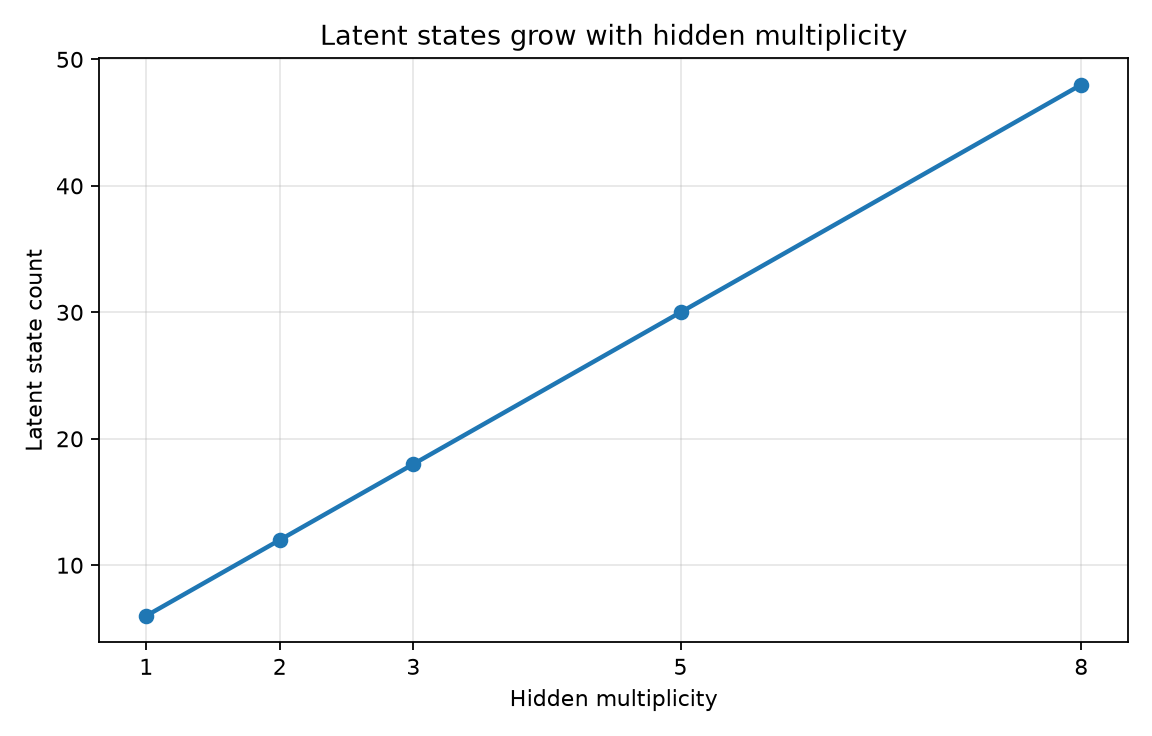
\includegraphics[width=0.86\textwidth]{original_repo_pngs/latent_state_count_vs_hidden_multiplicity.png}
\caption{Each hidden label adds six source states.}
\end{figure}

\begin{figure}[H]
\centering
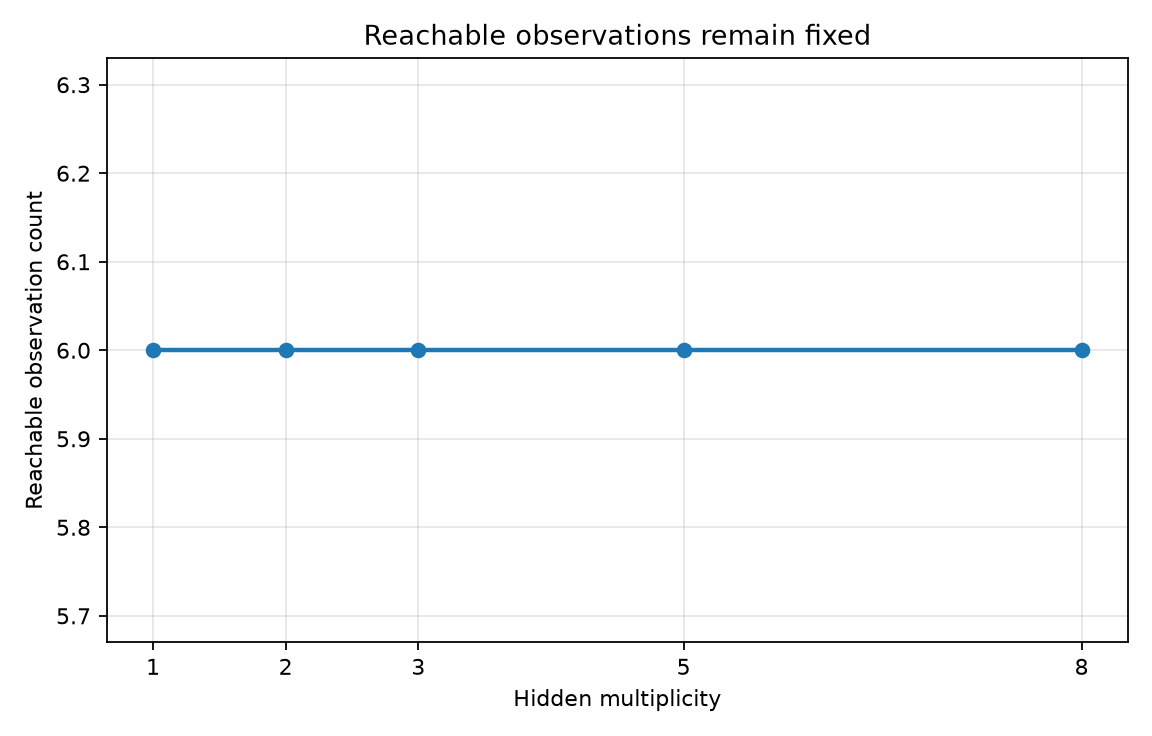
\includegraphics[width=0.86\textwidth]{original_repo_pngs/reachable_observation_count_vs_hidden_multiplicity.png}
\caption{The number of reachable observations stays at six as hidden multiplicity increases.}
\end{figure}

\begin{figure}[H]
\centering
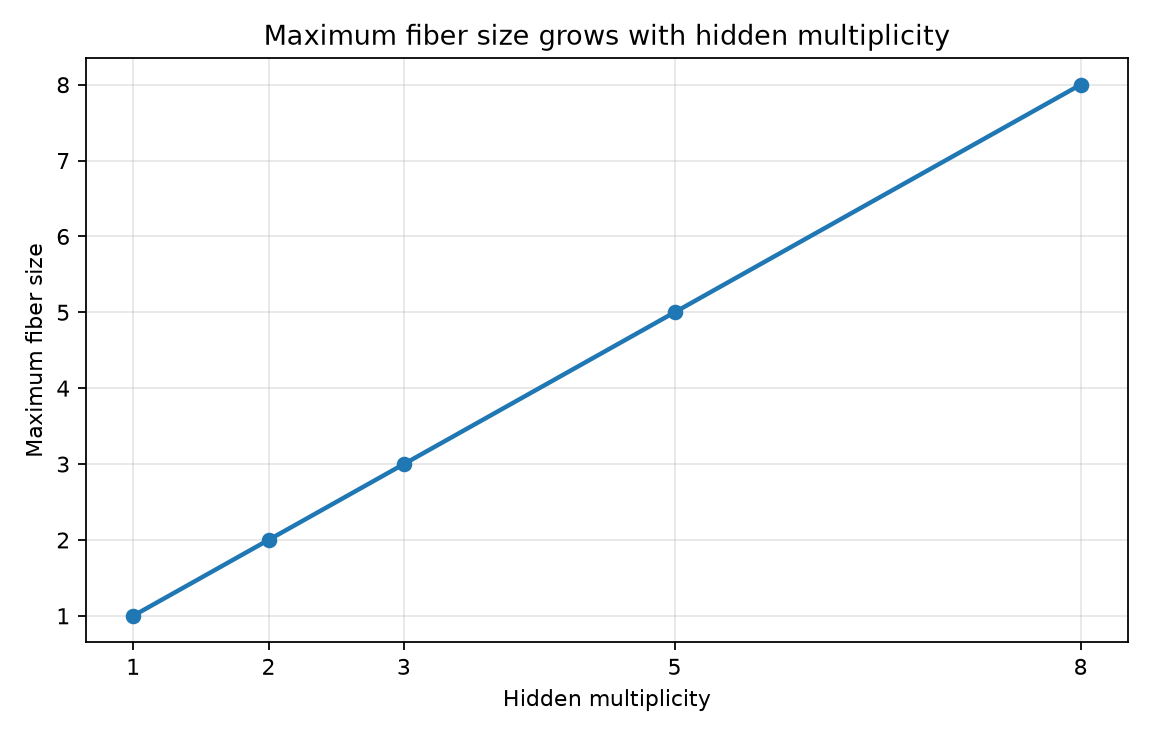
\includegraphics[width=0.86\textwidth]{original_repo_pngs/maximum_fiber_size_vs_hidden_multiplicity.png}
\caption{The maximum fiber size equals the number of hidden labels at each multiplicity.}
\end{figure}

\begin{figure}[H]
\centering
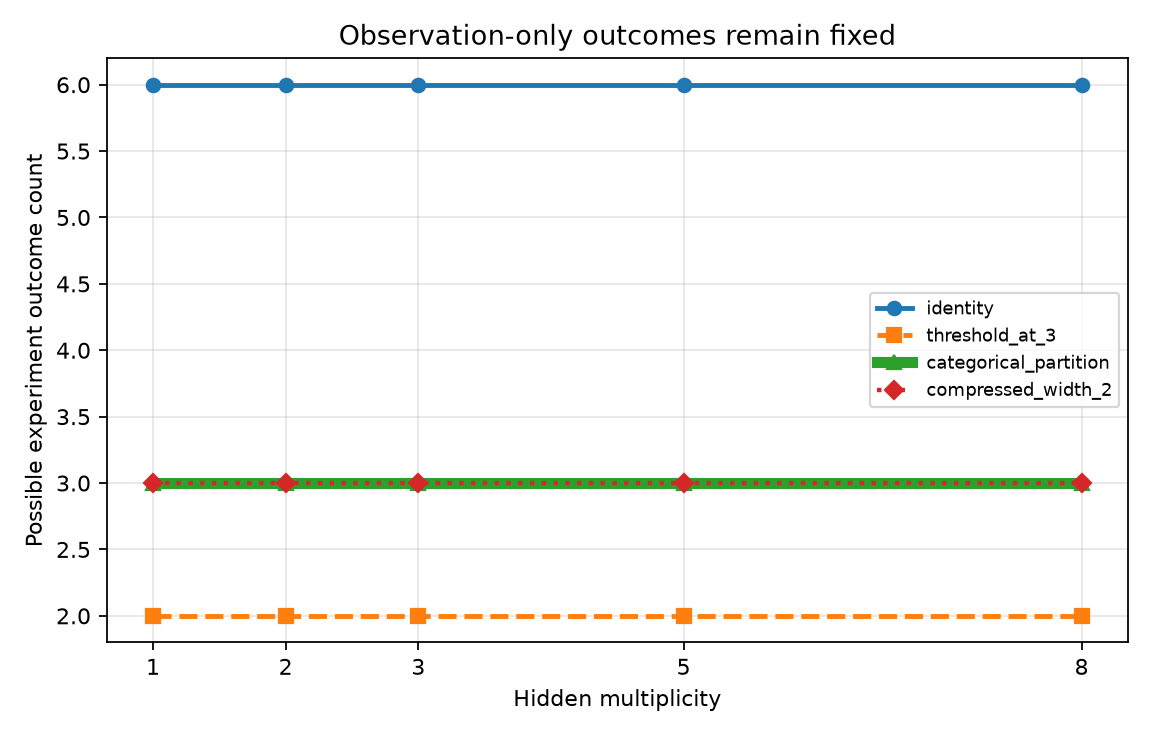
\includegraphics[width=0.86\textwidth]{original_repo_pngs/experiment_outcome_count_vs_hidden_multiplicity.png}
\caption{Each rule has a fixed number of possible outcomes across the six-output models.}
\end{figure}

\begin{figure}[H]
\centering
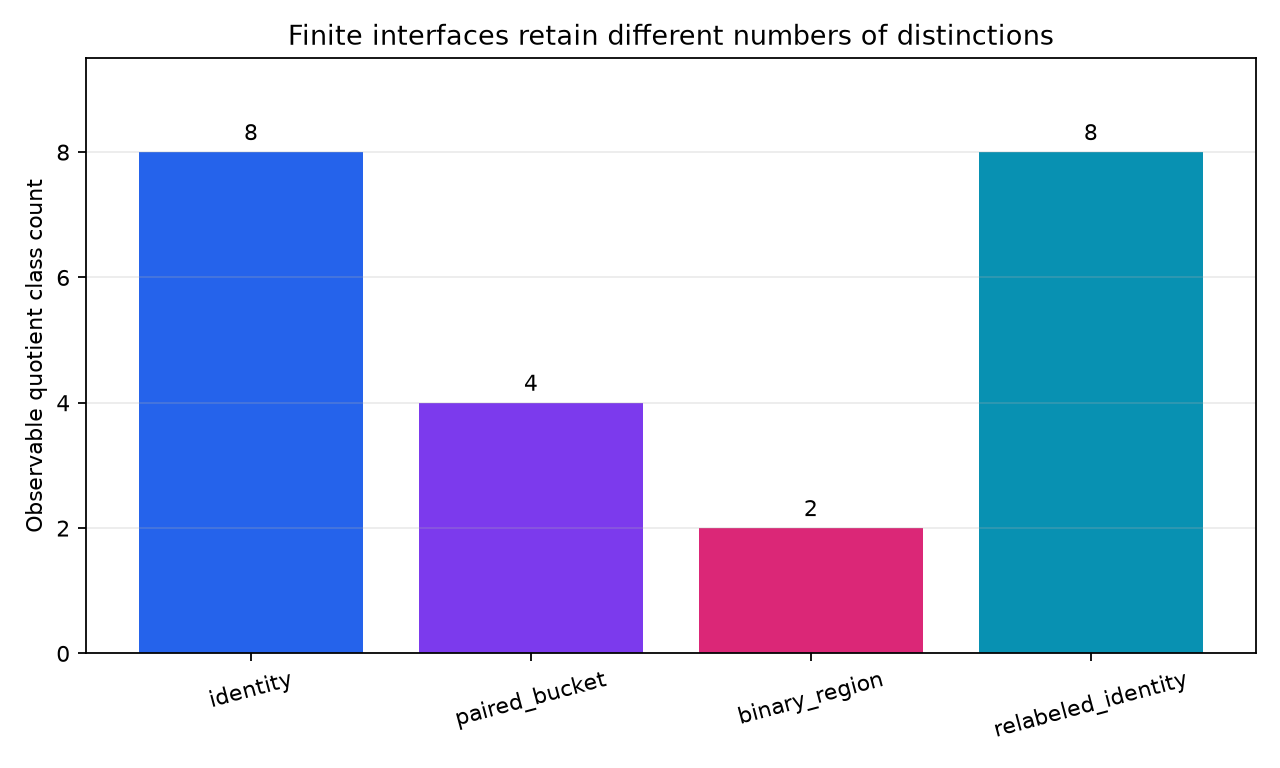
\includegraphics[width=0.90\textwidth]{original_repo_pngs/observable_quotient_size_by_interface.png}
\caption{Identity and relabeled identity retain eight classes. Paired buckets retain four and binary regions retain two.}
\end{figure}

\begin{figure}[H]
\centering
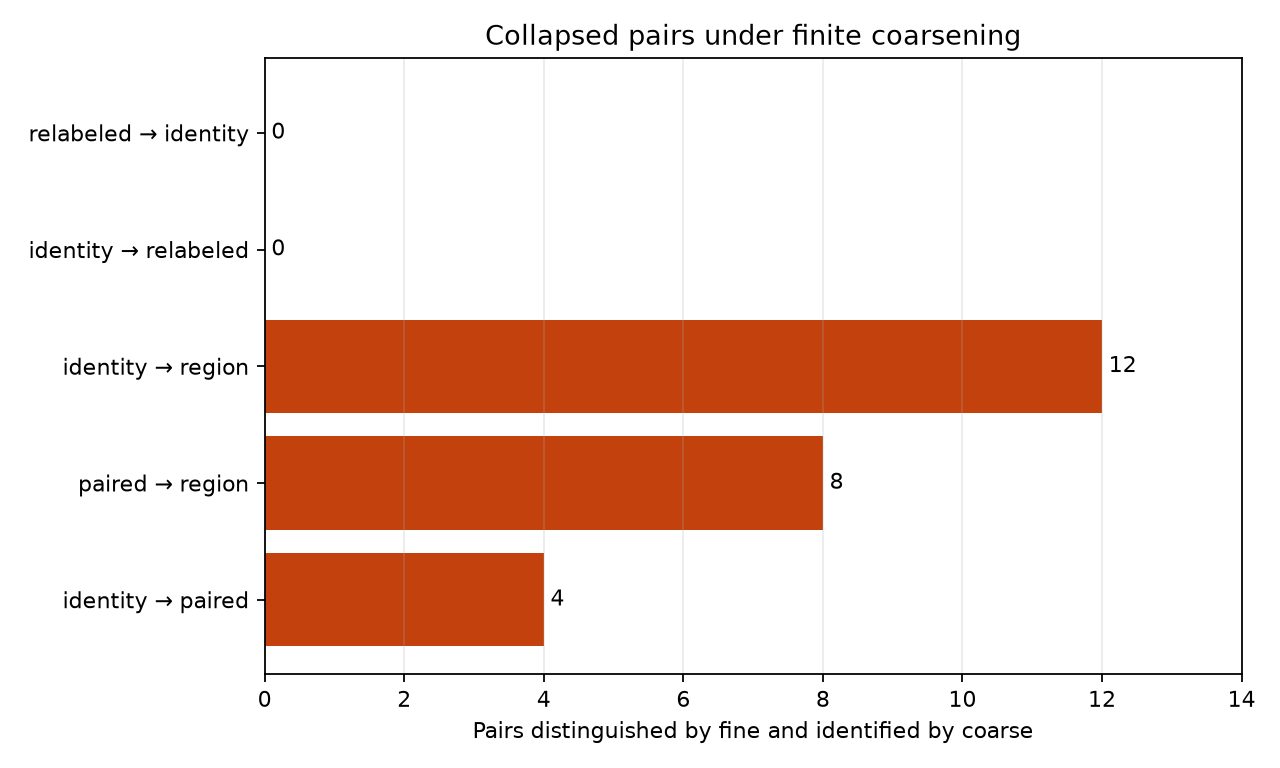
\includegraphics[width=0.90\textwidth]{original_repo_pngs/collapsed_pairs_by_refinement.png}
\caption{The three strict coarsenings merge four, eight, and twelve pairs, respectively. Relabeling merges none.}
\end{figure}
